
By changing just one line of code, you can control the speed at which the LED on your Arduino blinks.

\GOALS
This chapter introduces how we can give additional information to a procedure to control its behavior. 

\CODE

\lstinputlisting[caption=The {\procname blink} procedure is quite handy.,label=code:blink13]{code/blink13.occ}

% I'm starting to wonder if this is ``Discussion'', or something.. 
\PATTERNS
In the previous chapter, we saw the {\procname heartbeat} procedure. In this chapter, we changed line 2. In our first program, we used the \plumbing procedure called {\procname heartbeat} to blink the LED. In this chapter, we instead are using {\procname blink}, which lets us control both which LED we are blinking as well as the speed at which the LED blinks.

\begin{figure}[h]
  \begin{center}
    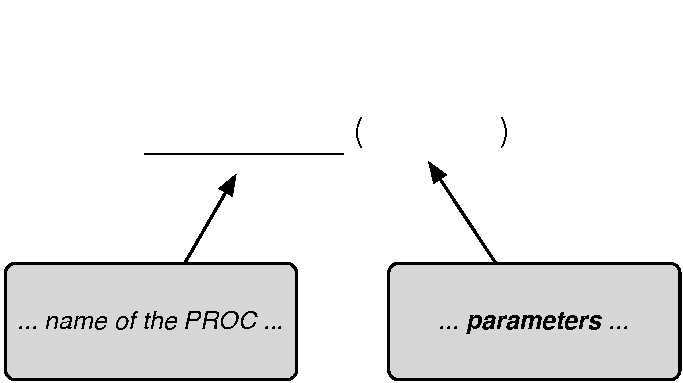
\includegraphics[width=\linewidth]{images/parameter-pattern}
    \caption{Parameters go inside the parentheses of a procedure call.}
    \label{pattern:parameters}
  \end{center}
\end{figure}

On line 2, we can see that a \PROCedure called {\procname blink} is being called. This is just like {\procname heartbeat}---the code for that procedure is provided by the \plumbing environment. However, instead of an empty set of parentheses, there is stuff in-between them. 

\begin{verbatim}
	blink (13, 500)
\end{verbatim}

These are called {\em parameters}. Parameters are values that we give to procedures that let them do different things based on the values we provide. For example, the first parameter to the procedure {\procname blink} is the number {\constant 13}. This tells the Arduino which bit it should be turning on and off. Technically, we would say that the pin to which the LED is attached is being driven \HIGH and \LOW. As we explore more of the basics of electronics, you'll come to understand why we say \HIGH and \LOW instead of ``on'' and ``off.''

The second parameter is the amount of time that we want to go by between when the LED is turned on and off. You might think that {\constant 500} is a rather large amount of time---until you realize that it is a value in {\em milliseconds}. The prefix {\em milli} means {\em one thousandth}. Therefore, 1000 milliseconds (or 1000ms) equals 1 second. Therefore, half of a second is 500ms, and a tenth of a second is 100ms. 

Parameters are always separated by a comma.

\section{Adding an LED}
You now have enough \plumbing code to add an LED to your Arduino, and control it {\em instead} of the LED on the board!

% XXX Replace me with a hand-drawn picture?
%\begin{figure}[h]
%  \begin{center}
%    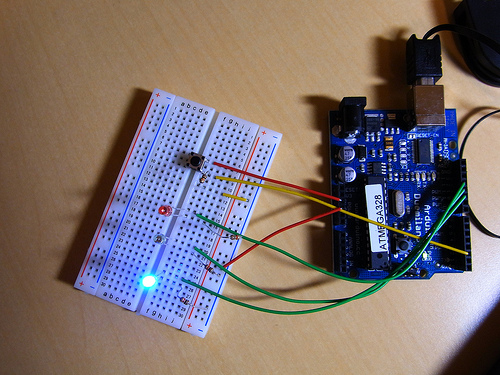
\includegraphics[width=\linewidth]{images/one-led}
%    \caption{Connect up one LED to your Arduino.}
%    \label{circuit:one-led}
%  \end{center}
%\end{figure}

Your Arduino will live at the center of a number of increasingly complex circuits. We call them {\em circuits} because they are a circular connection---a loop---that makes its way from a voltage source (often labeled {\code +5V} or {\code Vcc} in diagrams) through one or more electronic components back to ``ground'' (typically labeled {\code GND}). To connect up another LED, you're going to need:

\begin{enumerate}
	\item A breadboard
	\item An LED
	\item A 470\ohm resistor
	\item Some jumper wires
	\item Your Arduino
\end{enumerate}

We'll build the circuit up one step at a time. What we won't be doing is teaching you electronics---for that, we recommend you pick up a used copy of Horowitz and Hill's {\em The Art of Electronics}.\webnote{http://frank.harvard.edu/aoe/}{{\em The Art of Electronics}} We will, wherever possible, provide you with Wikipedia or wikiHow links that will help you understand what you're doing, but this is a book about programming with \plumbing, not the fundamentals of circuit design.

\subsection{The Breadboard}
The breadboard provides a foundation for building and testing small circuits. Breadboards come in many shapes and sizes; if you have a small Arduino kit, you might have a breadboard like that pictured in Figure~\vref{diagram:little-red-breadboard-connections}. Note that things in a column (on one side of the gutter) are connected, but things on opposite sides of the gutter are not. 

\begin{figure}[h!]
  \begin{center}
    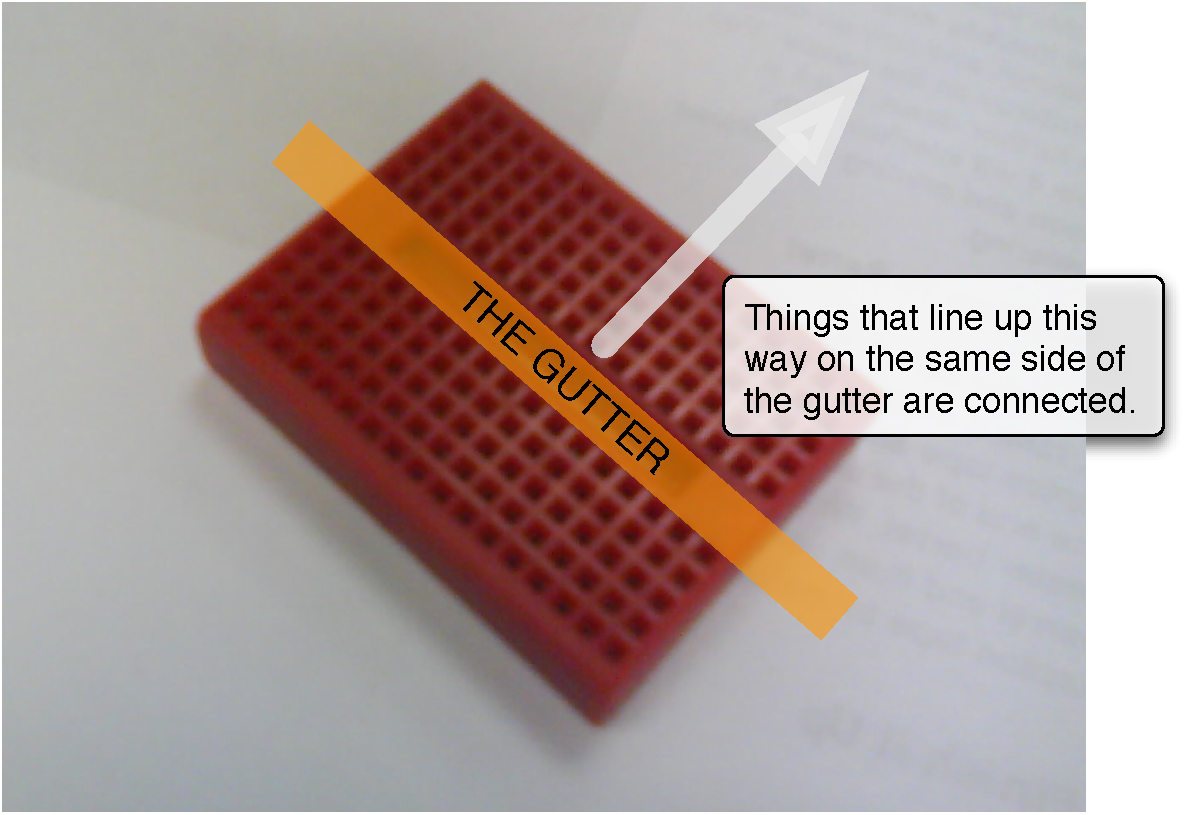
\includegraphics[width=0.8\linewidth]{images/little-red-breadboard-connections}
    \caption{How a breadboard works.}
    \label{diagram:little-red-breadboard-connections}
  \end{center}
\end{figure}

\subsection{The Arduino}
With the Arduino turned off (unplugged from the USB port), take a wire and connect it from pin 14 to one of the columns in the breadboard. Perhaps start with the left-most column, and we'll build our circuit from left-to-right.

\subsection{The Resistor}
If you plug your LED directly into an electronic device---even one as small as the Arduino---you might ``cook'' it. When you cook an LED, it typically flashes brightly once and never lights again. Therefore, we need a resistor to help limit the flow of current through our circuit, so the LED doesn't get fried. If you need a rule of thumb (which is not always correct!), a 1K\ohm resistor is typically more than enough to protect your LED.

Resistors are the little barrel-shaped things with different colored stripes on them. Those stripes tell you what resistance value they have.\webnote{http://en.wikipedia.org/wiki/Electronic_color_code}{the color codes on resistors} Plug one end of the 470\ohm resistor (Yellow Purple Brown Gold) into the same column of the breadboard as the wire you connected from the Arduino, and the other into an unused column further to the right. 

\subsection{The LED}
LEDs are a kind of diode. A diode is a device that only allows electric current to flow in one direction. Therefore, if you connect an LED up ``backwards,'' nothing will happen. If you connect it up correctly, current will flow, and it will light up. 

\begin{figure}[ht]
  \begin{center}
    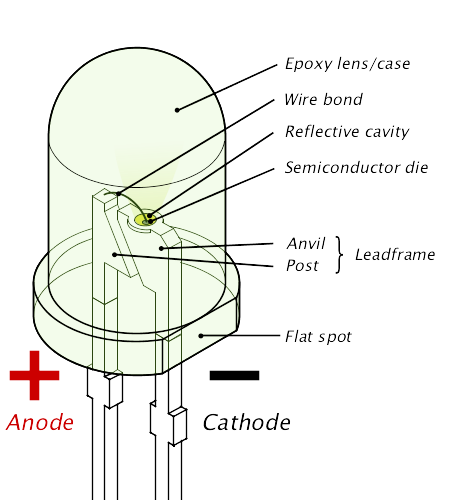
\includegraphics[width=0.5\linewidth]{images/led-internals}
    \caption{The internals of an LED.}
    \label{diagram:led-internals}
  \end{center}
\end{figure}

Because you have to connect it up the right way, some people say ``the long leg of the LED is the negative leg.'' This is true, but if your LED gets mangled, it becomes difficult to tell which leg is which. Instead, look at Figure~\vref{diagram:led-internals}, and find the ``anvil.'' The anvil is the larger of the two bits inside the LED, and it is {\em always} the negative side of the LED, meaning the ``post'' is {\em always} the positive side of the LED.\webnote{http://en.wikipedia.org/wiki/Led}{LEDs}

Plug your LED into the breadboard so that the positive side is in the same column as your resistor, and the negative side is in a column all by itself.

\subsection{Completing the circuit}
Lastly, to complete the circuit, connect the negative side of the resistor to the {\code GND} pin on your Arduino with a jumper wire. You should now have a complete circuit that looks like Figure~\vref{diagram:led-circuit-diagram}. Below this picture is the equivalent circuit diagram that you might find in a text on electronics; you can see the source of the current ({\code +5V}), the resistor (a squiggly line), the LED (the triangle with the arrows coming off of it), and ground. 

\begin{figure}[ht]
  \begin{center}
    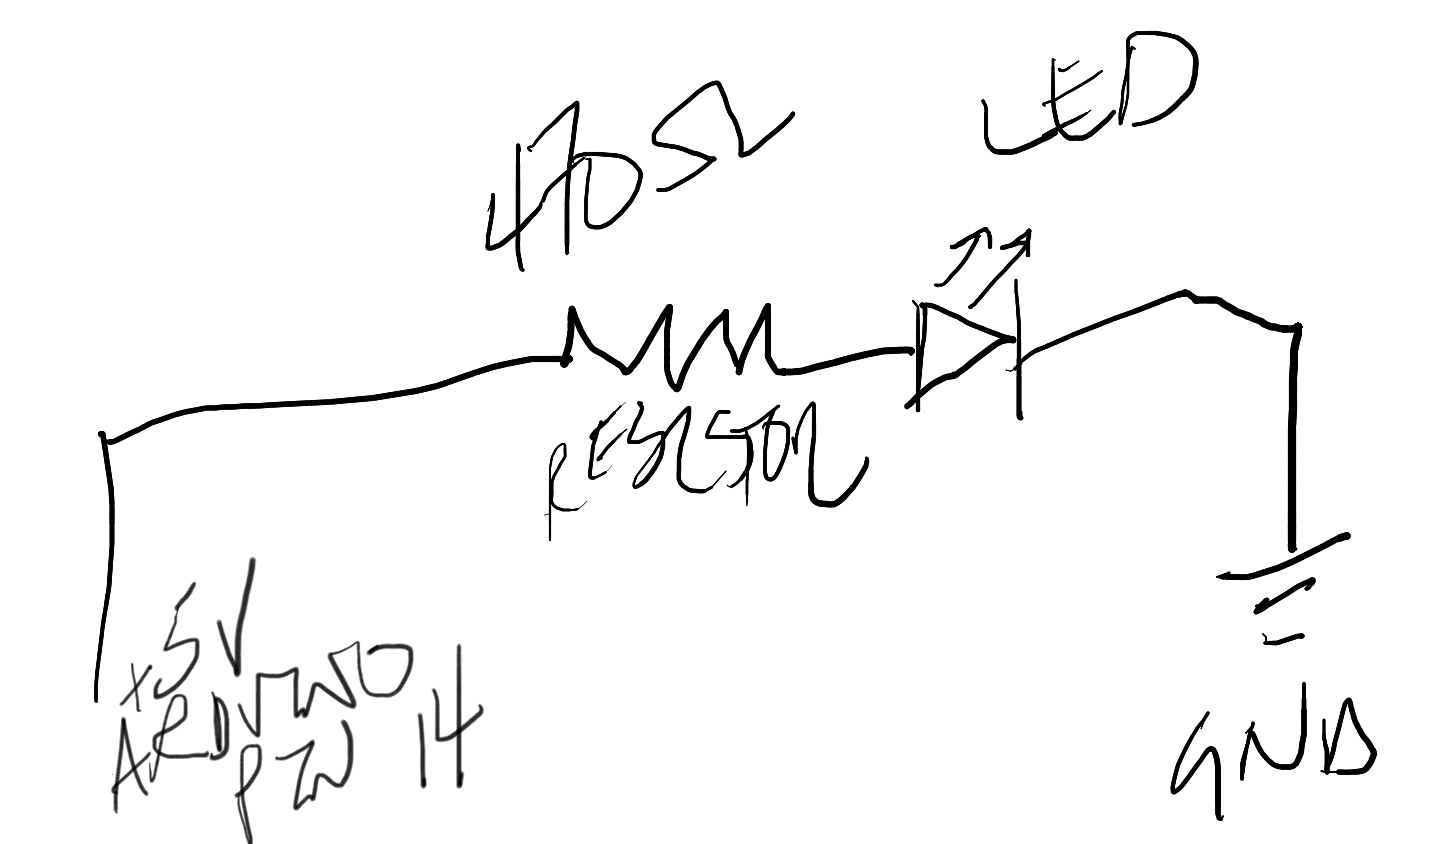
\includegraphics[width=0.8\linewidth]{images/led-circuit-diagram}
    \caption{The completed blinkenlight circuit.}
    \label{diagram:led-circuit-diagram}
  \end{center}
\end{figure}

Now, you should be able to plug in the USB cable, and type in the code from this chapter. If you compare the code in Listing~\vref{code:blink13} and the code in Listing~\vref{code:blink14}, you will see that we changed  one of the parameters to the procedure {\procname blink} on line 2. Instead of blinking pin {\constant 13}, we instead are asking the Arduino to blink pin {\constant 14}.

\newpage

\lstinputlisting[caption=Blinking an external LED on pin 14.,label=code:blink14]{code/blink14.occ}

If you've done everything correctly, you should now have an external LED blinking away!

\subsection{Faster blinkenlights!}
Once you've got it working, try playing with the second parameter to {\procname blink}. Currently we are using the value {\constant 500}. What happens if you make it higher? Lower?

\BREAKAGE
There are a number of things that can break in this chapter.

\subsection{Hardware}
You've completed your first circuit. However, you might have done something wrong, in which case, nothing will work. You can intentionally break a few things without damaging your Arduino or burning out your LED.

\begin{description}
	\item[Flip the LED]\ \\ 
	If you flip the LED around, it won't light. It won't burn out, either... but it won't work.
	\item[Wire wiggles]\ \\
	If you wiggle a wire out of place, you'll break the circuit. Then, nothing will work.
\end{description}

You can safely do each of these things, and see how your circuit fails to blink properly.

\subsection{Software}
There are quite a few ways you can break the software in this chapter---even though it is only three lines long!

\begin{description}
	\item[Wrong pin]\ \\
		If you forget to change the pin number from {\constant 13} to {\constant 14}, then you'll blink the wrong LED. Or, for that matter, if you blink pin {\constant 15}, nothing will appear to happen at all.
	\item[Crazy parameters]\ \\
	Try replacing the number {\constant 14} with {\code FOURTEEN}. See what happens. 
	\item[Too many parameters]\ \\
	Try using a parameter list like {\code 13, 14, 500}. That is, your code would look like:
	\begin{verbatim}
		blink (13, 14, 500)
	\end{verbatim}
	\item[Parameters too big]\ \\
	The parameter for the speed of the LED blink is an integer---a whole number without any decimal parts, if you prefer. Computers can only keep track of numbers that are so big (or small). How big can you make the blink speed? 
	\item[Blink too fast]\ \\
	What happens if you make the blink speed too small (e.g.~zero)?
	\item[Fractional blinking]\ \\
	What happens if you try and blink the LED every 100.5ms?
\end{description}

Remember, keeping track of the mistakes you make helps you know how to deal with them when you encounter them in your own programs later.


		



 


